\documentclass{article}
\usepackage{graphicx}
\usepackage{amssymb}

\title{Inverse Kinematics for Human Fingers}
\date{2016/10/26}
\author{3858103 - Ricky van den Waardenburg}

\begin{document}
\maketitle
\newpage

\section{Introduction}

Human finger ik solver. C++ OpenGL SDL2 SDL2TTF Finger assigned to me : little finger.

\section{Mathematical model}

\begin{figure}[h!]
\centering
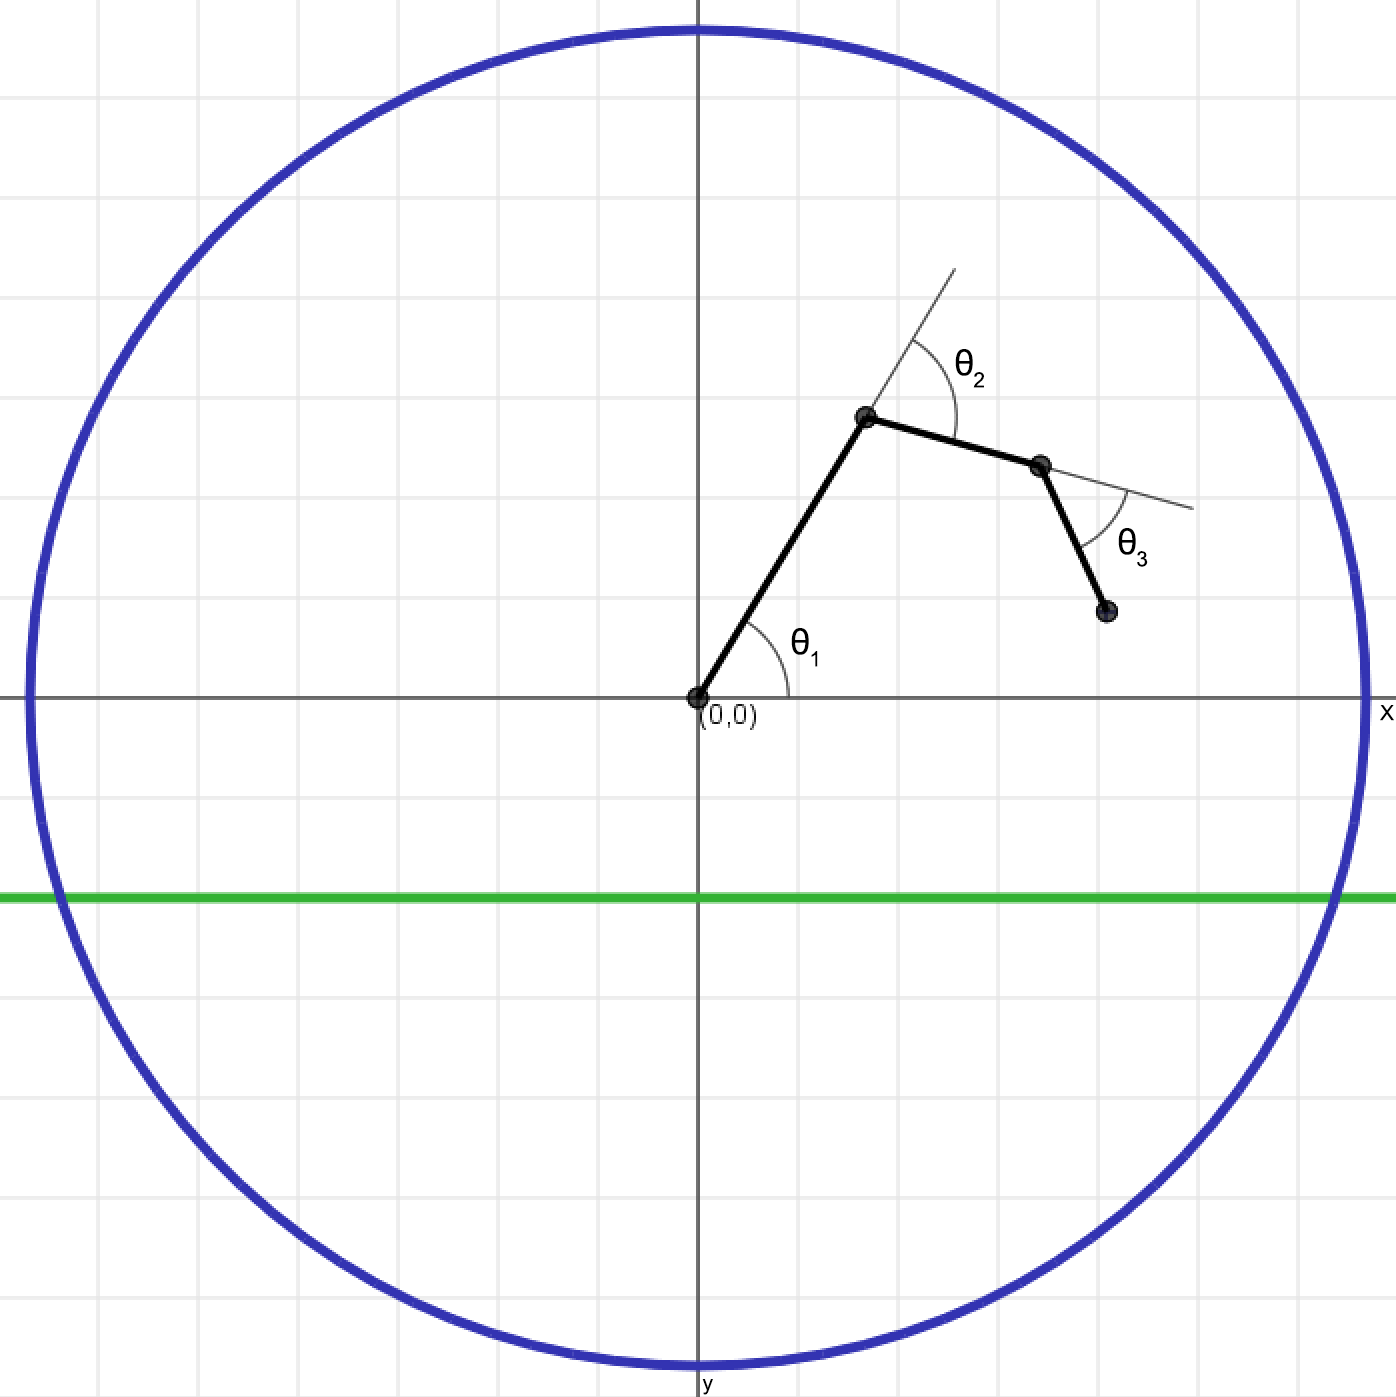
\includegraphics[scale=0.15]{situation.png}
\caption{Situation sketch.}
\end{figure}

\begin{table}[h!]
\centering
\caption{Little finger link lengths}
\label{my-label}
\begin{tabular}{lll}
\hline
\textbf{Link}                 & \textbf{Length} (in mm) &  \\\hline
Proximal phalanx     & 32.7           &  \\
Intermediate phalanx & 18.1           &  \\
Distal phalanx       & 16.0           & \\\hline
\end{tabular}
\end{table}

Initial model. Three bones represented by links. The proximal phalanx, intermediate phalanx and distal phalanx. TABLE OF LENGTHS HERE.
Three 1-DOF joints which axes are parallel to and as such rotate in the z-axis. Angle limits.
$ – \pi / 3 ≤ \theta M ≤ \pi / 3, –2 \pi / 3 ≤ \theta P ≤ 0, and –2 \pi / 3 ≤ \theta D ≤ 0$
All motions of the finger take place in the (x,y) plane.

Three (n = 3) joints rotate in z-axis only, as such everything is in (x, y) space.

Unbounded object O x, y, z in R y + 2 $<=$ 0. Infinite plane parallel to the x-axis at height y = -2.

\subsection{Forward kinematics}

Forward kinematics equations and experimentation. Transformation matrices.

0T1
1T2
2T3

0T3 = 0T1 * 1T2 * 2T3 = matrix

q = theta1 theta2 theta3


\subsection{Forward kinematics with joint constraint}

Reworked forward kinematics equations and experimentation.

2T3 = different

\subsection{Inverse kinematics}

Jacobi-matrix for reworked forward kinematics equations. Other IK related equations.

\section{Implementation of inverse kinematics solver}

Link to github. Description of ik solver

\section{Experimentation}

Initial guess is important. Alpha is important for accuracy. Edge cases for initial guess.  

\end{document}